\documentclass[openany,12pt]{book}
\usepackage[utf8]{inputenc}
\usepackage[spanish]{babel}
\usepackage{slashbox}
\usepackage{graphicx}
\usepackage{booktabs}
\usepackage{svg}
\usepackage{pdfpages}
\usepackage[backend=bibtex,citestyle=numeric,sorting=none]{biblatex}
\usepackage{csquotes}
\usepackage{float}
\usepackage[bottom]{footmisc}

\title{Desarrollo de un sistema para la clasificación y análisis de fuentes de ruido en entornos urbanos aplicando modelos basados de aprendizaje automático}

\author{Carlos David Camacho\\Esteban Elías Romero\\Codirector: Oscar Esneider Acosta\\Director: Carlos Enrique Montenegro}
\date{Marzo de 2021}

\addbibresource{bibliografia/articulos.bib}


\begin{document}
\maketitle
\tableofcontents

\part{Anteproyecto}


\chapter{Introducción}


%Ideas orden párrafo:

%1. Ruido y sus efectos en la salud

El oído humano es un órgano sensorial, el cual se mantiene activo todo el tiempo, Jimena Martinez \cite{JimenaMartinezLlorente2015}
 afirma que:
 
A diferencia de la visión, que se apaga por las noches, el oído es un sentido de alarma, que siempre está activo para detectar situaciones de peligro. Por lo tanto, el oído no se puede cerrar como se cierran los ojos cuando se duerme y siempre percibe todo lo que le llega.(P. 6).
 
Este órgano tiene la capacidad de recibir estímulos desde el exterior. Cada estimulo a los que se refiere anteriormente puede interpretarse como sonido, sobre el cual el mismo autor afirma que: 

El sonido es un cambio de presión del aire, que se mueve como una ola circular a partir de la fuente, [...] Estos cambios de presión entran en el canal auditivo, se transmiten del aire al tímpano del oído, que a su vez mueve los huesecillos del oído medio. Los huesecillos funcionan como un amplificador mecánico y pasan los movimientos al caracol, donde hacen moverse el líquido linfático que contiene Este, al moverse estimula los células ciliadas que a su vez reaccionan generando impulsos nerviosos que se envían al cerebro(P. 6).

Con base a la información anterior podemos introducir un término que es la base del contexto del problema y este trabajo, el ruido, el cual citando nuevamente al autor afirma que: ``se define como la sensación auditiva inarticulada generalmente desagradable, molesta para el oído. Técnicamente, se habla de ruido cuando su intensidad es alta, llegando incluso a perjudicar la salud humana.". De forma similar la directiva europea 2002/49/CE \cite{EUROPEO2002} en el artículo 3 define el ruido como 
``Sonido exterior no deseado o nocivo generado por las actividades humanas, incluido el ruido emitido por los medios de transporte, por el tráfico rodado, ferroviario y aéreo y por emplazamientos de actividades industriales".

Atendiendo al análisis anterior, el ruido, es un problema que afecta a la salud, en el artículo ``Hipoacusia por ruido: Un problema de salud y de conciencia pública"\cite{Ugalde2000} se afirma que:

Los principales efectos adversos sobre la salud reconocidos por la Organización Mundial de la Salud y otros organismos como la Agencia de Protección Ambiental de EEUU, y el Programa Internacional de Seguridad Química son : Efectos auditivos (discapacidad auditiva incluyendo tinnitus), dolor y fatiga auditiva, perturbación del sueño, efectos cardiovasculares, respuestas hormonales, disminución rendimiento en el trabajo y la escuela, molestia, interferencia con el comportamiento social, interferencia con la comunicación oral

A nivel urbano (la zona de estudio de este trabajo) el ruido es producido por diversas fuentes como autos, actividades de construcción, entre otros.  Un ejemplo es la ciudad de Bogotá (Colombia) que de acuerdo con la Secretaria Distrital de Ambiente\cite{Ambiente} ``En Bogotá D.C. las fuentes móviles (tráfico rodado, trafico aéreo, perifoneo) aporta el 60\% de la contaminación auditiva. El 40\% restante corresponde a las fuentes fijas (establecimientos de comercio abiertos al público, PYMES, grandes industrias, construcciones, etc)".

En este orden de ideas, se requiere tener un sistema que permita la clasificación y el análisis en tiempo real de fuentes ruidos en un ambiente urbano. 
 

\chapter{Glosario}
\begin{itemize}
    \item Advanced Encryption Standard (AES): ``Es un algoritmo de cifrado simétrico aplicado por NIST (Instituto Nacional de Estándares y Tecnología)"\cite{RFC3826}.
    \item Concurrencia: ``Es la tendencia de las cosas a producirse al mismo tiempo en un sistema"\cite{contconcurrency}.
    \item Fisiología: ``Ciencia que tiene por objeto el estudio de las funciones de los seres orgánicos"\cite{rae_2020}.
    \item Free Lossless Audio Codec (FLAC): ``Formato de audio similar al MP3, pero sin pérdidas, [...] el audio se comprime en FLAC sin pérdida de calidad"\cite{flac}.
    \item Frecuencia: ``Medida del número de veces que se repite un fenómeno por unidad de tiempo [...]fenómenos ondulatorios, tales como el sonido y las ondas electromagnéticas"\cite{euFrecuencia}.
    \item Edge-Computing: ``Es un tipo de informática que ocurre en la ubicación física del usuario, de la fuente de datos, o cerca de ellas"\cite{redHatEC2020}.
    \item Mel Frequency Cepstral Coefficients (MFCC): ``Representan la amplitud del espectro del habla de manera compacta, esto los ha vuelto la técnica de extracción de características más usada en reconocimiento del habla"\cite{MFCC}.
    \item Message Queue Telemetry Transport MQTT: ``Es un protocolo de mensajería estándar de OASIS para Internet de las cosas. Está diseñado como un transporte de mensajería de publicador/subscriptor extremadamente liviano"\cite{mqtt}.
    \item Programación concurrente: ``Rama de la informática que trata de las
    técnicas de programación que se usan para expresar el paralelismo entre tareas y para
    resolver los problemas de comunicación y sincronización entre procesos"\cite{concurrencia_2020}.
    \item Señal Análoga: ``Es una señal continua en la que una cantidad variable en el tiempo (como voltaje, presión, etc.) representa otra variable basada en el tiempo"\cite{arrowAnalogous}
    \item Señal digital: ``Una señal digital es una señal que representa datos como una secuencia de valores discretos"\cite{monloganalog}.
    \item Serverless: ``Es una manera de crear y ejecutar aplicaciones y servicios sin tener que administrar infraestructura [...] no tiene que aprovisionar, escalar ni mantener servidores para ejecutar aplicaciones, bases de datos y sistemas de almacenamiento" \cite{aWsSl}.
    \item Smart city: ``Ciudad que utiliza tecnología digital para conectar, proteger y mejorar la vida de los ciudadanos. Los sensores de IoT, las cámaras de video, las redes sociales y otras entradas actúan como un sistema nervioso, proporcionando al operador de la ciudad y a los ciudadanos una retroalimentación constante para que puedan tomar decisiones informadas"\cite{ciscoSC}.
    
    \item Rivest, Shamir y Adleman (RSA): ``Es un sistema de cifrado de clave pública, [...] cualquiera puede enviar un mensaje cifrado secreto a un receptor designado. Esto es sin que haya ningún contacto previo utilizando solo información disponible públicamente "\cite{mitRSA}.
    
    \item Virtual Private Network(VPN): ``Red privada que utiliza una red pública para conectar sitios o usuarios remotos entre sí. En vez de utilizar una conexión real dedicada como línea arrendada, utiliza conexiones "virtuales" enrutadas a través de Internet desde la red privada de la empresa hacia el empleado o el sitio remoto"\cite{ciscoVPN}.
    \item Visión artificial: ``Tiene como objetivo generar descripciones inteligentes y útiles de escenas y secuencias visuales, así como de los objetos que aparecen en ellas, mediante la realización de operaciones sobre imágenes y vídeos"\cite{mathworksVA}.


    
\end{itemize}

\chapter{Planteamiento del problema}




El ruido en los últimos años ha tomado mayor importancia al ser considerado unos de los principales contaminantes del aire \cite{Murphy2014}. De hecho, estudios de la Unión Europea han determinado que el ruido es el segundo factor que más aporta a la contaminación del aire en ese continente por debajo solamente del material particulado \cite{EuropeanEnvironmentalAgency2014}. Adicionalmente, diferentes estudios estudios han demostrado los efectos en la salud a nivel fisiológicos y psicológicos que genera el ruido ambiental en las personas \cite{King2003}, \cite{Recio2016}. En estos efectos se pueden mencionar cefalea, problemas cardiovasculares, estrés, entre otros.

Es así como, el ruido es generado por fuentes sonoras las cuales aportan a la contaminación acústica, muchas de ellas debido a la actividad humana. Como fuentes de ruido en entornos urbanos se pueden mencionar dos principales categorías. La primera, corresponde a fuentes de ruido estáticas en donde industrias, bares, comercio, entre otros, generalmente, radian energía acústica de forma esférica en el ambiente. La segunda categoría corresponde a fuentes de ruido móviles que son asociadas a fuentes de transporte terrestre, aeronáutico y férreo \cite{Murphy2014}. 

En el contexto colombiano, el ruido ambiental es regulado con la resolución 627 de 2006 \cite{Ministeriodeambienteviviendaydesarrolloterritorial2006}. En ella se establece la forma como se deben realizar los estudios de ruido ambiental en el país y los niveles máximos permisibles dependiendo del uso del suelo. De igual manera, en esta resolución se determina que es obligación de las corporaciones autónomas regionales, con base en los estudios de ruido ambiental, establecer medidas para controlar sus niveles.

Adicionalmente, para realizar medidas de gestión de ruido ambiental es necesario conocer el aporte de cada fuente de ruido. Es así como, la aplicación de técnicas de aprendizaje automático para clasificar y estimar la contribución de los medios de transporte al ruido ambiental en términos de indicadores acústicos, mediante la clasificación del tráfico pesado, liviano (motos y automóviles) y aéreo es relevante. Lo anterior, toma importancia en la medida que la principal fuente de ruido en grandes ciudades suelen ser los medios de transporte \cite{omidvari2009effects}. 

Al lograr caracterizar, categorizar y separar las fuentes de ruido ambiental móviles, se permitiría conocer el aporte de cada fuente de forma independiente lo cual aportaría información a las entidades estatales encargadas de realizar los planes de gestión de ruido, para lograr niveles acústicos adecuados según el uso de suelo de un territorio. De esta manera, se plantea la siguiente pregunta problema:

¿Cómo se pueden clasificar las fuentes de ruido en un entorno urbano?


\chapter{Objetivos}

\section{Objetivo general}
\begin{itemize}
    \item Desarrollar un sistema que permita la clasificación y análisis estadístico de las fuentes de ruido en entornos urbanos aplicando modelos de aprendizaje automático.
\end{itemize}
\section{Objetivos específicos}
\begin{itemize}
% responder esto en cada objetivo: que, para que, como. Por que.
% estudiar algoritmos 
% definir los requisitos que debe cumplir el algoritmo o métricas.
%Decir por que se algoritmo.
    \item Definir el modo de adquisición y procesamiento del sonido, para determinar las herramientas de hardware y software necesarias por medio de un estudio del estado del arte de sistemas similares.
    \item Definir las métricas y requerimientos para la selección de algoritmos basados en aprendizaje automático para la clasificación de sonidos encargados de generar las inferencias sobre el audio, por medio de revisión documental matemática aplicada a la evaluación de la precisión de dichos algoritmos.
    \item Desarrollar una arquitectura de software que permita la inferencia sobre los datos de  audio, interacción con distintos modelos de aprendizaje automático, y el acceso a los resultados, por medio del estudio del estado del arte de arquitecturas, implementación de prácticas en el marco de la cultura DevOps, desarrollo de pruebas y prototipos.
    \item Implementación de una interfaz de usuario para el análisis estadístico de los resultados por medio de tecnologías que permitan el desarrollo ágil dentro de un marco de trabajo. 
    % probar.
    
\end{itemize}

\chapter{Justificación}
El ruido es un factor que ha tomado gran importancia en el país debido al aumento de quejas que se presentan ante las entidades gubernamentales. En el caso de Bogotá se estima que al mes hay 300 quejas por ruido ante la Secretaría Distrital del Medio Ambiente (SDA) \cite{Beltran2008}.

Adicionalmente, en ciudades del mundo que desde hace varios años han tratado problemáticas de ruido, la tendencia es disponer de sistemas de monitoreo ubicados en puntos estratégicos en donde se conoce, a través de mapas de ruido tradicionales, existen niveles altos de contaminación acústica \cite{Bellucci2018}. Estas estaciones entregan indicadores de ruido ambiental durante las 24 horas del día, permitiendo conocer de una mejor manera el comportamiento dinámico del ruido. 

Lo anterior, se integra al concepto de Smart Cities en donde a través del uso de WNS (Wireless Sensor Networks) y transductores de bajo costo se han venido implementado redes que capturan datos de ruido de forma continua \cite{Asensio2017}, los cuales son transmitidos a centros de almacenamiento en donde son convertidos en información. Inicialmente, esta información solo proporcionaba indicadores acústicos (Leq, L10, L90, entre otros) para describir el ruido.

Sin embargo, últimamente aplicando técnicas de aprendizaje automático es posible identificar la fuente de ruido y separarla de otras fuentes para poder realizar un análisis diferencial y establecer el aporte de cada fuente al problema de ruido \cite{Imoto}.

Con base en lo anterior, al disponer de un sistema que permita clasificar fuentes de ruido en un entorno urbano, permitiría a las entidades encargadas de tomar acciones en medida de ruido, como lo son las corporaciones autónomas regionales, centrar sus refuerzos en el diseño de medidas de mitigación para estas fuentes de ruido.

\chapter{Estado del arte}


La temática del ruido en ambientes urbanos ha marcado todo camino de desarrollo de herramientas tecnológicas con las que se puede observar y tratar este problema desde diversos ángulos (observación de los niveles de contaminación, puntos de mayor presencia de sonidos específicos, sistemas  información, etc). Dichas herramientas implementan diversos métodos que permiten solucionar algún problema en específico de la temática, como por ejemplo la clasificación de sonidos, lo cual se puede lograr por medio de herramientas basadas en Deep Learning. A continuación se dará mención a sistemas y herramientas que buscan hacer frente a la temática o un problema especifico dentro del rango de la misma: 


\section{SONYC}En la ciudad de Nueva York existe una iniciativa para el monitoreo, análisis y mitigación de la contaminación acústica urbana. SONYC consiste en un sistema tipo CPS (cyber-physical system)  el cual se encarga de recolectar datos en forma de audio de distintos lugares de Nueva York para que luego sean procesados para que posteriormente se pueda realizar un análisis de ruido mediante frameworks para la visualización \cite{Bello2018}. En la Figura 6.1 se encuentran los tres elementos claves los cuales se describen a continuación:

\begin{itemize}
\item Recolección de datos (Sensing): los datos se obtienen por medio de dispositivos ubicados en varios lugares de Nueva York y consisten en una Raspberry Pi equipada con un módulo de micrófono de sistemas micro electromecánicos (MEMS). Estos dispositivos generan fragmentos de audio de 10 segundos durante un período de tiempo limitado que posteriormente se comprime con el codificador FLAC, luego se asegura la conexión utilizando AES y RSA. Los nodos se comunican a través de una red privada virtual (VPN)\cite{Bello2018}. 
\item Análisis : El análisis de datos se enfoca en el desarrollo de técnicas de procesamiento de datos e interfaces para la visualización de la información para que pueda ser interpretada tanto de por usuarios con experiencia como aquellos que carecen de ella. Urbane (Figura 6.2) es una de las tecnologías de visualización sobre las que trabaja el grupo de trabajo de SONYC, consiste en un mapa 3D que permite computación en tiempo real, integración y visualización de múltiples flujos de datos\cite{Bello2018}.
\item Actuación: Refiere a técnicas que podrían mitigar. SONYC menciona el efecto de las penalizaciones sobre alguna entidad (empresa o individuo) que de acuerdo al número de ellas puedo reflejar un resultado en cuanto a mitigación a corto y largo plazo. Este análisis de acuerdo con SONYC podría reducir los costos en las intervenciones y aumentar la mitigación del ruido\cite{Bello2018}.
\end{itemize}


\begin{figure}[H]
\centering
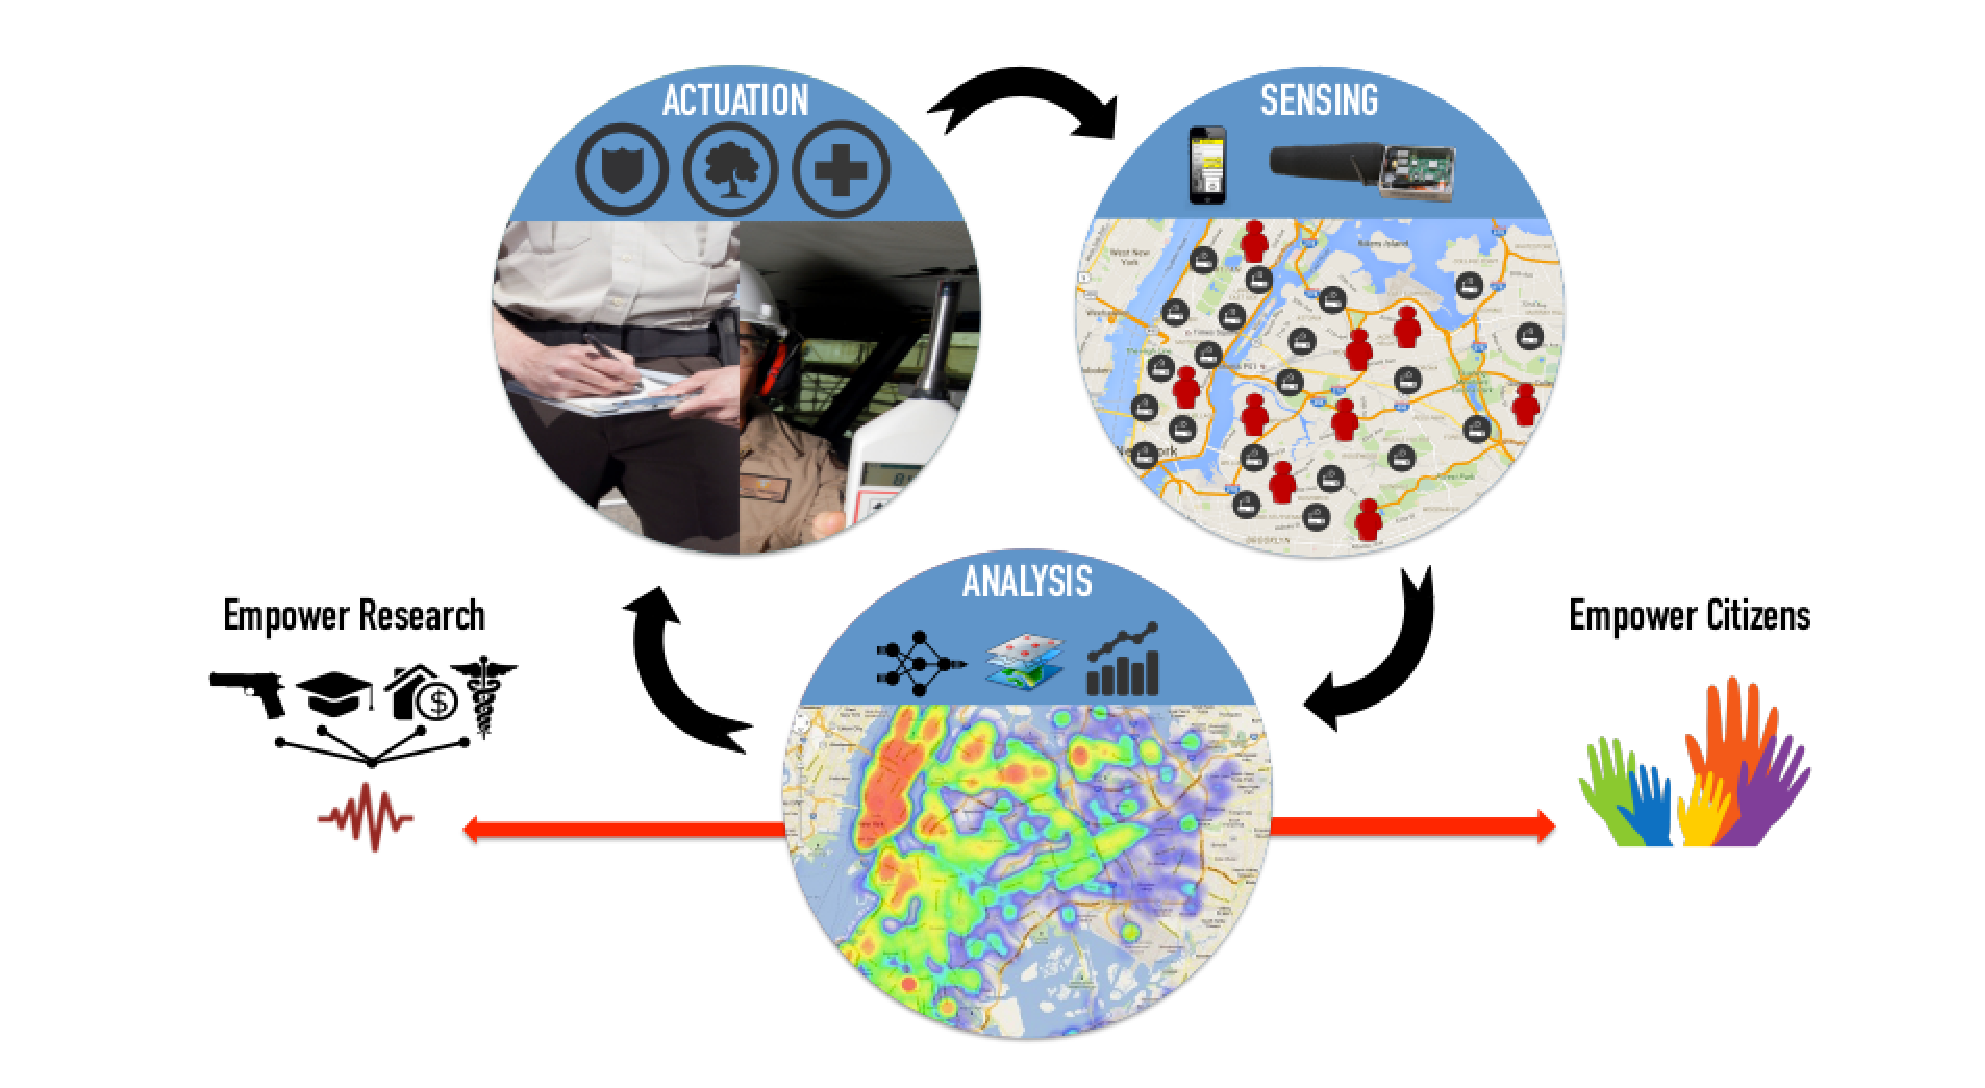
\includegraphics[width=\linewidth]{bibliografia/Imagenes/SONYC.eps}
\caption{SONYC: A System for the Monitoring, Analysis and Mitigation of Urban Noise \cite{Bello2018}}
\end{figure}


\begin{figure}[H]
\centering
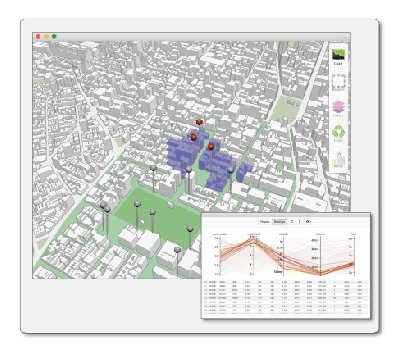
\includegraphics[width=0.6\linewidth]{bibliografia/Imagenes/Urbane.eps}

\caption{Urbane: A 3D framework to support data driven decision making in urban development \cite{Bello2018}}
\end{figure}

\section{Stadtlärm}
Es un sistema de monitoreo de ruido mediante sensores distribuidos (sistemas embebidos) que almacenan y procesan datos en forma de audio, estos son procesados posteriormente en servidores que despliegan servicios para aplicaciones de usuarios. Opera sobre una arquitectura basada en servicio (Broker) utilizando MQTT como protocolo de comunicación \cite{Abeer2019}. Este proyecto como puede observarse en su arquitectura (Figura 6.3) tiene 3 componentes elementales que conforme con el autor se describen a continuación:

\begin{itemize}
    \item Aplicación y visualización: La información es representada en 3D y es usada para diseñar y verificar modelos de ruido-espacio \cite{Abeer2019},\cite{DigitalMediaTechnology2016}.
    \item Unidad de recolección de datos (Acoustic Sensor Units): Se compone de una Raspberry Pi 3, un micrófono MEMS integrado en un PCB y un slot tipo M2 para un módem inalámbrico, y sistemas de protección de agentes externos\cite{Abeer2019}.
    \item Procesamiento de datos (Central Server) : El modelo de clasificación consiste en redes neuronales convolucionales basadas en el modelo de paradigma VGG entrenado para la clasificación entre nueve clases\cite{Abeer2019}.
\end{itemize}

\begin{figure}[H]
\caption{Stadtlärm Project Architecture \cite{Abeer2019} }
\centering
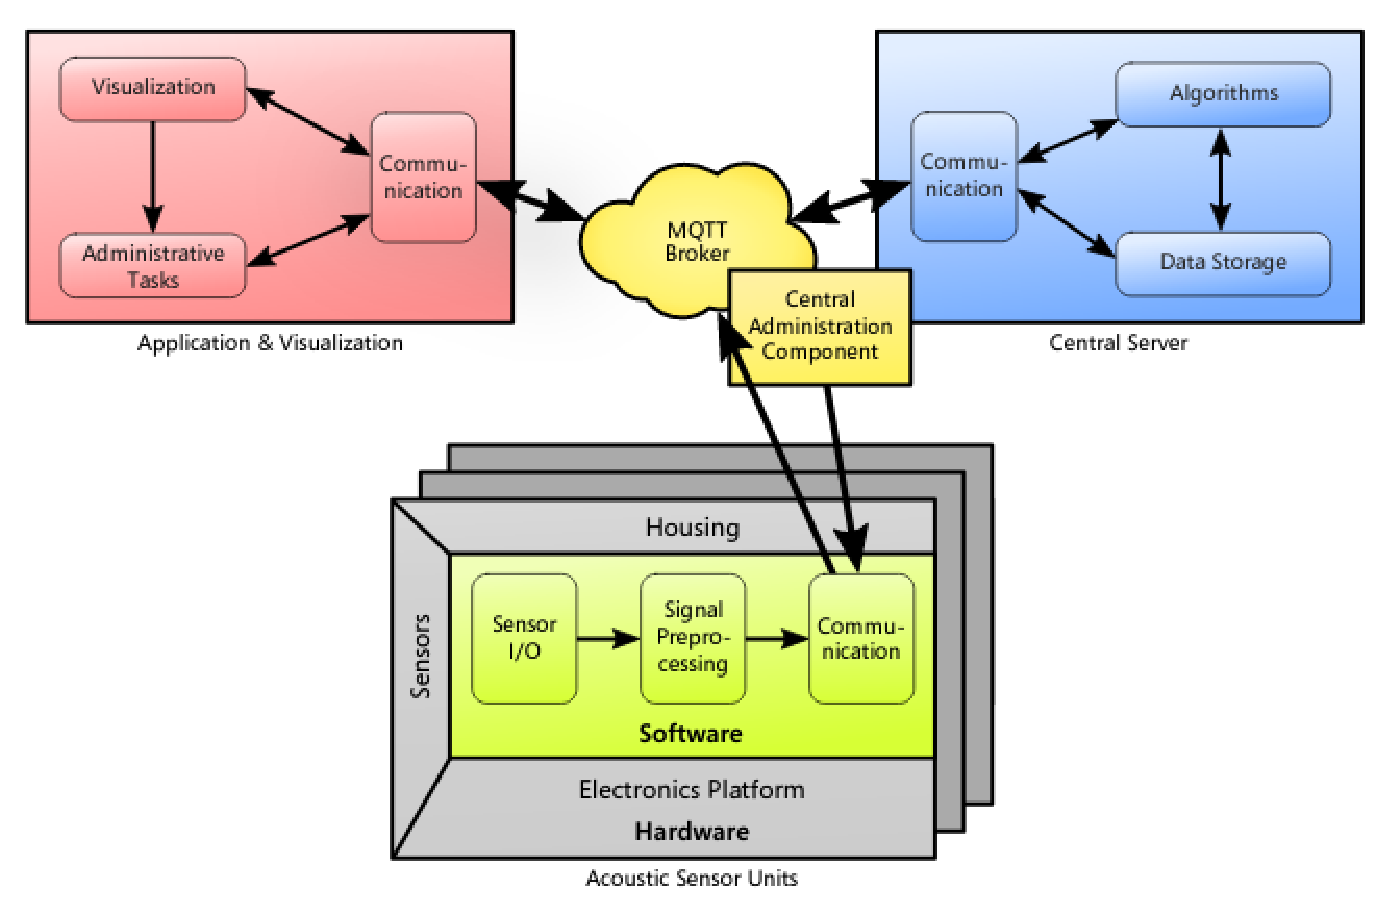
\includegraphics[width=\linewidth]{bibliografia/Imagenes/stadtlarm_arch.eps}
\end{figure}

\section{Dynamap}

Es un proyecto para la actualización de mapas de ruido en tiempo real mediante el uso de mapas básicos de ruido provenientes de diferentes fuentes actualizados mediante una red de sensores de bajo costo en el área de mapeo \cite{Bellucci2018}. Lo mapas básicos son escalonados para proveer un mapa completo del área (Figura 6.4), algunas características se describen a continuación:

\begin{itemize}
    \item Sensores de bajo costo: Existen dos tipos de sensores el primero un sensor de alta capacidad de computo (HCCS) capaz de realizar varias operaciones entre ellas el análisis espectral sobre las señales. El segundo un sensor es de baja capacidad con un limitado número de operaciones y se localiza en los lugares donde no se requiera análisis espectral\cite{Bellucci2018}.
    \item Algoritmo ANED: Es un algoritmo para discriminar sonidos anómalos o aquellos que no sean generados por tránsito rodado. El algoritmo puede identificar entre las siguientes categorías : rodado, ruido de fondo y ruidos anómalos. Los últimos están divididos en 18 categorías\cite{Bellucci2018}.
    \item Aplicación NOISEMOTE : Es un software para la publicación de datos históricos y en tiempo real, se utiliza herramientas estadísticas para mostrar tendencias, valores promedios, entre otros \cite{Bellucci2018}.
    \item web-GIS : Es un software para reescalar mapas básicos de ruido en función de los niveles de ruido detectados por los sensores. Con ellos se genera un mapa completo de un área, los resultado son posteriormente publicados\cite{Bellucci2018}.
\end{itemize}


\begin{figure}[H]
\centering
\includegraphics[width=\linewidth]{bibliografia/Imagenes/dynamap.eps}
\caption{The DYNAMAP project - (Dynamic AcousticMapping - Development of low cost sensors networks for real time noise mapping\cite{Bellucci2018}}
\end{figure}

\section{A Machine Learning Driven IoT Solution for Noise Classification in Smart Cities}

Es un proyecto para la clasificación de ruidos urbanos aplicando IoT y un algoritmo de clasificación basado en SVM (Support Vector Machine) y K-nearest neighbors llegando a una precisión en el rango entre 85\% y 100\%, entrenado utilizando el dataset UrbanSound8K y MFCC (Mel Frequency Cepstral Coefficients) para la extracción de carácteristicas. Como plataforma IoT se utiliza la Raspberry Pi Zero W, un dispositivo de bajo costo y del tamaño de una tarjeta de crédito. Un objetivo de este proyecto es usar edge-computing por lo tanto el algoritmo de clasificación se ejecuta en la plataforma IoT. 

Con base en lo anterior una de las características Edge-computing permiten que el flujo de datos pueda distribuirse hacia puntos cercanos del origen de datos lo cual disminuye la necesidad de realizar el procesamientos de todos los datos en un único centro de datos, añadiendo a esto la capacidad del algoritmo mencionado de ejecutarse en dispositivos de bajo costo con lo cual el dispositivo de procesamiento de datos y origen de datos son el mismo. 

\chapter{Marco referencial}
%que es machinelearning, como se interpreta el sonido por el microfono/audi que es un API, Servidor sistemas embebidos, conectividad


\section{Marco conceptual}

\subsection{Sonido}
Se puede entender el sonido como la sensación que percibe el oído ante las perturbaciones en un medio, al momento de tocar una guitarra el sonido es producido por la vibración de las cuerdas, de una manera similar ocurre con los demás instrumentos musicales, en las bocinas, el sonido es producido por la vibración de una membrana que empuja el aire del medio y genera estas ondas. \cite{fisica_conceptual}
\subsection{Ondas sonoras}

Onda longitudinal que se propaga por un medio elástico generando cambios de presión o densidad produciendo lo que conocemos como sonido, según \cite{fisica_serway} las ondas sonoras según su frecuencia pueden ser clasificadas en 3 tipos 
\bigskip

\begin{itemize}
    \item\textbf{1. Ondas infrasónicas} Tienen frecuencias por debajo del intervalo audible, no pueden ser interpretadas por el oído humano.
    \item\textbf{2. Ondas audibles} son aquellas que puede percibir el oído humano, se encuentran en aparatos electrónicos, instrumentos musicales, etc.
    \item \textbf{3. Ondas ultrasónicas} Son aquellas ondas que tienen frecuencias superiores al intervalo audible. 
\end{itemize}


\subsection{Interpretación del sonido por medio de equipos electrónicos}

Desde que se inventó el fonógrafo en el siglo 19, la humanidad ha podido almacenar los sonidos para ser escuchados en cualquier momento, \textit{<<Las ondas sonoras se registraban en los primeros fonógrafos al codificarlas formas de onda sonoras como variaciones en la profundidad de un surco continuo cortado en una delgada hoja enrollada alrededor de un cilindro.>>}\cite{fisica_serway}, para poder procesar una onda sonora los dispositivos actuales transforman la señal original expresada en términos del tiempo x(t) a una señal expresada en términos de la frecuencia X(f), es decir la señal pasa de ser una onda continua a ser discreta(creando una representación por medio una muestra de la amplitud por cada índice discreto\cite{audioCoding}) tal y como se puede observar en la Figura \ref{sonido_continuo_disctreto}, esta señal discreta puede ser almacenada en medios electrónicos como cds, archivos de audio, discos de vinilo, entre otros 

\begin{figure}[H]
\centering
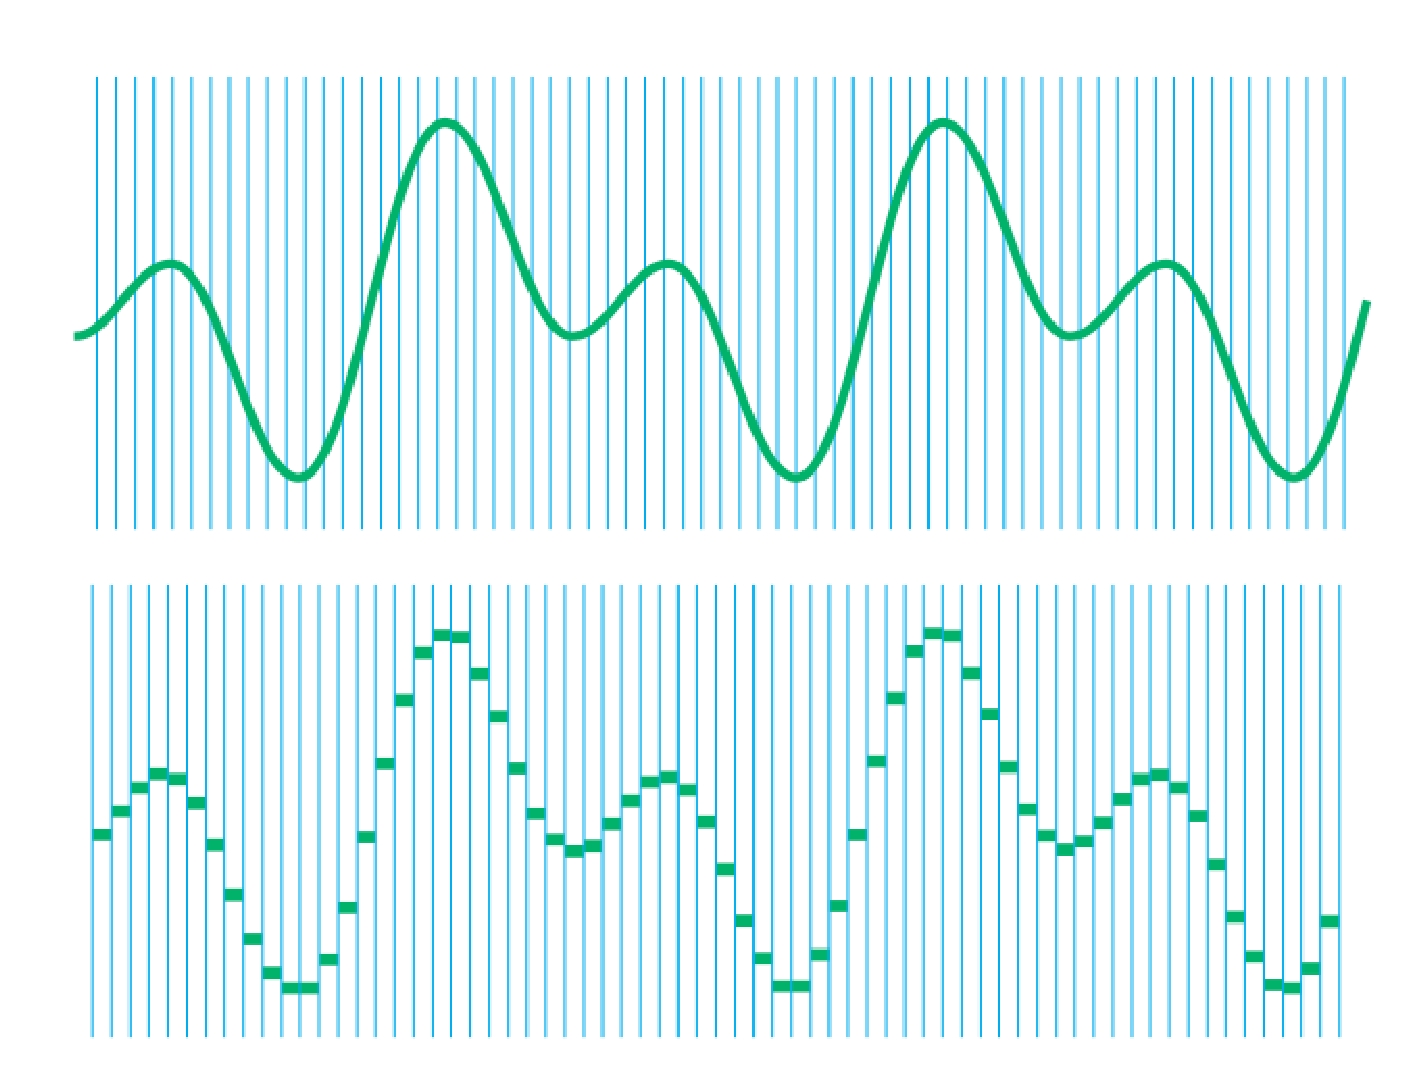
\includegraphics[width=0.7\linewidth]{bibliografia/Imagenes/transformacion.eps}
\caption{ imagen tomada de  \cite{fisica_serway}}
\label{sonido_continuo_disctreto}
\end{figure}

Posteriormente, la señal es transformada nuevamente de un espacio discreto a un espacio continuo para su correcta interpretación por parte del oído humano, este proceso trae consigo una disminución en la calidad del audio original, para estos procesos se hace necesario usar técnicas como la Transformada de Fourier y su transformada inversa. A continuación, en la figura \ref{sonido_digital} se observa el diagrama de bloque que representa el proceso de transformación de audio digital.
 
\begin{figure}[H]
    \centering
    \includegraphics[width=\linewidth]{bibliografia/Imagenes/transformacion2.eps}
    \caption{imagen tomada de \cite{audioCoding}}
    \label{sonido_digital}
\end{figure}
 
 


\subsection{Contaminación auditiva}

Este tipo de contaminación esta presente en todas las ciudades del mundo y es causada por diversos factores como la musica a volumen excesivo, el trafico, los aeropuertos, el comercio, entre otros. se considera un sonido como ruido ``cuando interfiere con actividades normales como dormir, conversar, o altera o disminuye la calidad de vida'' \cite{Agency}, estos ruidos pueden causar afectaciones a la salud\cite{ScientificAssistant1981}  ,El ministerio de ambiente de la ciudad de Bogotá ha publicado los efectos que el ruido causa en las personas \cite{Ambiente} 
\begin{itemize}
    \item{Estrés.}
    \item{Pérdida del sueño (insomnio).}
    \item{Ansiedad.}
    \item{Depresión.}
    \item{Cambios en el comportamiento (conductas agresivas).}
    \item{Baja Productividad.}
\end{itemize}
En particular y bajo la normatividad colombiana se encuentran las siguientes resoluciones relacionadas con los eventos sonoros  \cite{Ambiente}

\begin{itemize}
\item     ``Resolución No. 627/06 MAVDT: se adopta la norma nacional de emisión de ruido y ruido ambiental (parámetros permisibles, procedimientos técnicos y metodológicos para  la medición de ruido, presentación de informes, y otras disposiciones)'' \cite{Ambiente}, en esta resolución se establecen las unidades de medida para: 

\begin{itemize}
    \item[-] presión sonora: Pascal.
    \item[-] niveles de presión sonora: decibles.
\end{itemize}

También se reglamenta el uso correcto de los instrumentos de medición(sonómetro, aerómetro) así como su correcta calibración. Además se establecen los estándares Máximos Permisibles de Niveles de Ruido Ambiental como se observan a continuación.

\begin{figure}[H]
\centering
\includegraphics[width=\linewidth]{bibliografia/Imagenes/tablaNiveles2.eps}
\caption DB máximos permisibles de niveles de ruido ambiental {\cite{Ambiente}}
\end{figure}

\item     ``Resolución DAMA No. 185/99: establece condiciones generales para la obtención de permisos de perifoneo en el Distrito Capital'' \cite{Ambiente}.

\item     ``Resolución DAMA No. 832/00: establece la clasificación empresarial por impacto sonoro UCR que permite valorar las industrias y establecimientos, respecto a su nivel de generación de ruido.'' \cite{Ambiente}. 

\end{itemize}

\subsection{Inteligencia artificial en la clasificación del sonido}

En el campo de Inteligencia artificial, se han obtenido gran cantidad de logros relacionados con lo que un sistema computacional puede realizar, estos van desde máquinas que pueden competir con humanos en juegos de mesa\cite{Montesino2019}, autos que apoyan su conducción como el proyecto OpenPilot \cite{openPilot} el cual es uno de los mas importantes en el área de la conducción autónoma, análisis de información en diferentes campos por ejemplo en \cite{dornadula_credit_2019} mediante técnicas de aprendizaje de máquina se buscan patrones de comportamiento en los datos que registrados por cada una de las transacciones de compras en canales electrónicos. Así mismo, se encuentran sistemas basados en técnicas de aprendizaje de máquina para la clasificación de eventos sonoros como las diferentes técnicas de inteligencia artificial realizan un proceso similar al del cerebro humano con el fin de construir ``inteligencia". A continuación se observa como la información de archivos (datos binarios) es transformada en lo que se conoce como inteligencia 

\begin{figure}[H]
    \centering
    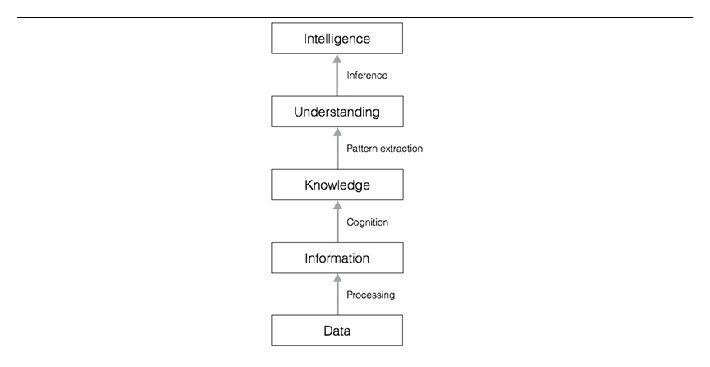
\includegraphics[width=\linewidth]{bibliografia/Imagenes/InteligenceTransform.eps}
    \caption{imagen tomada de \cite{alberto_artasanchez_artificial_nodate}}
\end{figure}

Las ramas de la inteligencia artificial se pueden clasificar de muchas maneras, en \cite{alberto_artasanchez_artificial_nodate} podemos encontrar una manera general para clasificar los diferentes algoritmos según cada aspecto relevante, un algoritmo se puede clasificar:

\begin{itemize}
    \item Según su método de aprendizaje:
    \begin{itemize}
        \item [-]    algoritmos de aprendizaje supervisados
        \item [-]    aprendizaje no supervisados
        \item [-]    aprendizaje por refuerzo
    \end{itemize}
    \item Según su función
    \begin{itemize}
        \item [-] (ANI) Inteligencia artificial estrecha: se caracteriza por realizar una tarea especifica de una muy buena manera, ratreo de paginas, juegos de mesa
        \item [-] (AGI) Inteligencia artificial General: pueden realizar cualquier tarea que un humano realiza por ejemplo conducir
    \end{itemize}
    \item Según su similitud con acciones Humanas: se caracterizan en las acciones que buscan suplir de la capacidad humana estos pueden ser 
    \begin{itemize}
        \item [-] Visión artificial
        \item [-] Aprendizaje
        \item [-] Procesadores de lenguaje natural
    \end{itemize}
\end{itemize}


Las redes neuronales artificiales son una de las técnicas mas frecuentemente usadas, estas se fundamentan una abstracción del procesamiento que realiza el cerebro humano, estas son capaces de crear un modelo con el fin de detectar los patrones presentes en un conjunto de datos y así realizar una clasificación adecuada de cada uno de los ejemplares de este conjunto. En cuanto a su arquitectura están divididas por la unión de distintas capas, se debe tener claro que una neurona es vista como la unidad mínima de procesamiento.

La neurona es la unidad básica de procesamiento dentro de una red neuronal. Cuentan con conexiones de entrada a través de los cuales reciben estímulos externos, la neurona realizará un cálculo interno y determinará una salida. 

Internamente el perceptrón realiza una suma ponderada de las entradas asignando a un valor de intensidad, también denominado peso. El cálculo interno busca que a partir de las entradas, los pesos se ajusten permitiendo determinar la salida esperada. Esto se denomina fase de entrenamiento de las neuronas. A continuación se observa la representación gráfica de una neurona.
 \begin{figure}[H]
    \centering
    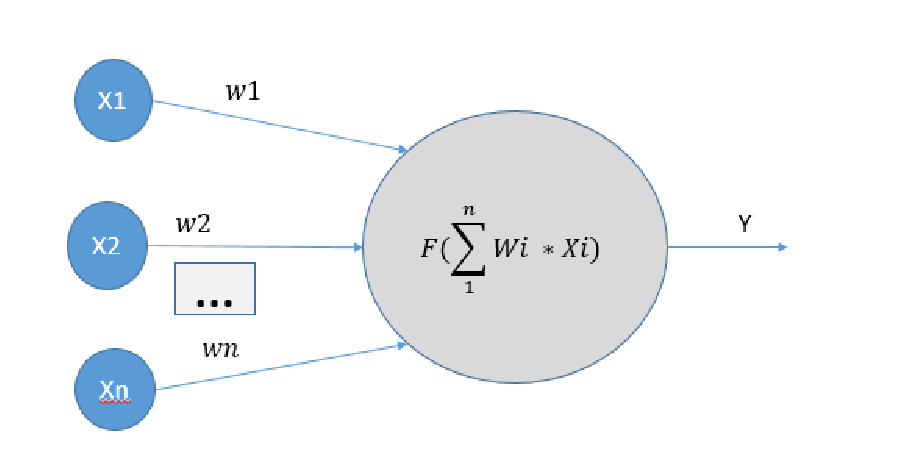
\includegraphics[width=0.8\linewidth]{secciones/Imagenes/neurona.eps}
    \caption{Neurona}
\end{figure}


Para la clasificación de audio el conjunto de datos para el entrenamiento consiste en una serie de grabaciones de eventos sonoros previamente etiquetados que ajustaran el modelo predictivo para identificar las características de los archivos de nuevos audio, finalmente basándose en las características se realiza un análisis para determinar el ejemplar a que conjunto de datos puede pertenecer.


En cuanto a los avances de inteligencia artificial como precedente encontramos el evento <<DCASE challenge>>\cite{Dc} en el cual anualmente se realiza un desafió con el fin de analizar diferentes eventos sonoros, además se encuentran los reportes técnicos de cada uno de los algoritmos implementados.\footnote{puede verse los resultados del evento del año  2020 en el siguiente enlace

\url{http://dcase.community/challenge2020/task-sound-event-localization-and-detection-results}
}.


\subsection{Arquitectura basada en Micro servicios}

En el mundo del desarrollo de software se crea la necesidad de comprender el mundo real traduciéndolo a un nivel de sistemas siempre buscando siempre un alto nivel de abstracción para esto, se utilizan diferentes enfoques como Arquitectura Orientada en servicios (SOA) o arquitectura de micro servicios. 

La arquitectura SOA busca crear sistemas por medio de conectar distintos componentes de software por medio de interfaces, esta arquitectura presenta aplicaciones mas seguras, integración con otros componente, aumento en el tiempo de entrega de los sistemas, sin embargo, esta si esta aplicación debe responder ante una gran cantidad de usuarios podría colapsar ya que es construida como una unidad (monolito),  

En la actualidad el software debe evolucionar a los cambios ágilmente. Por ejemplo, se debe responder ante una gran cantidad de usuarios o debido al dinamismo del mundo moderno la lógica del negocio se ve modificada, además de que abre la posibilidad de existencia de componentes transversales a la organización que pueden ser utilizados por diferentes áreas de negocio.

\begin{figure}[H]
    \centering
    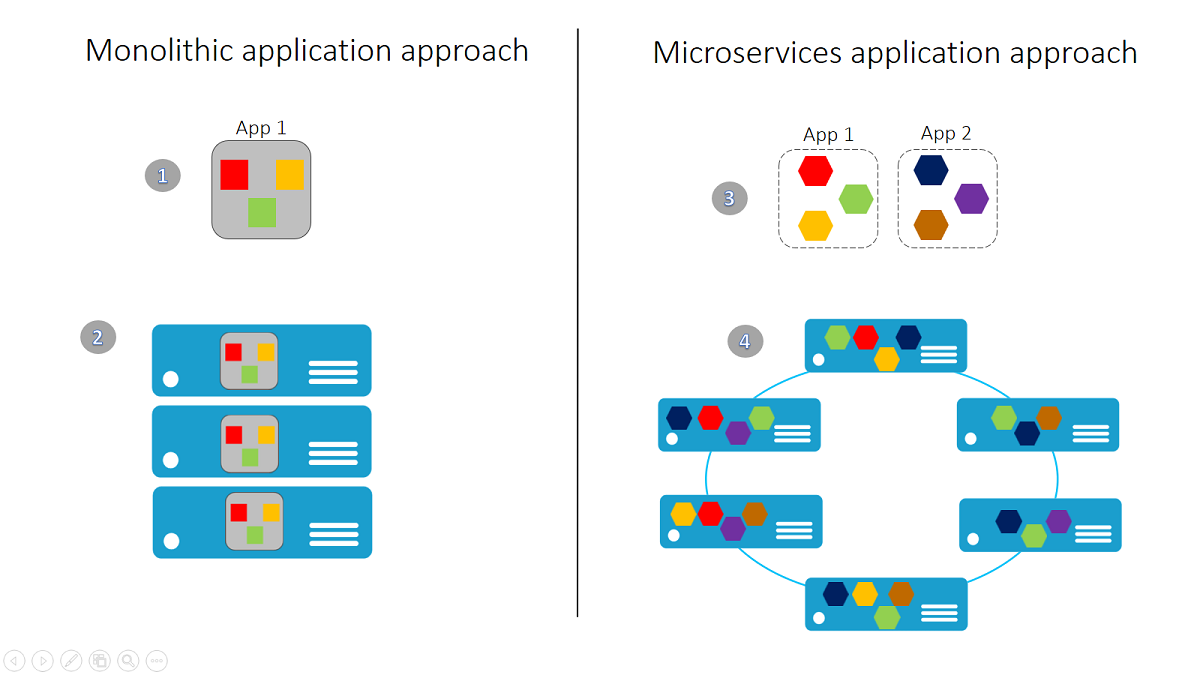
\includegraphics[width=0.8\linewidth]{bibliografia/Imagenes/monolithic-vs-micro.eps}
    \caption{imagen tomada de \cite{microservicios}}
\end{figure}


Los micro servicios presentan las siguientes ventajas frente a una arquitectura monolítica 

\begin{itemize}
    \item Se piden realizar cambios rápidamente
    \item Se implementan distintas tecnologías sin afectar el negocio, debido a que los servicios pueden ser desarrollados en  cualquier lenguaje de programación se puede elegir una tecnología adecuada para cada requerimiento
    \item Apoya la reutilización de componentes, distintas áreas del negocio pueden comunicarse para consumir un mismo servicio evitando así que cada área genere 2 veces el mismo componente.
\end{itemize}

\subsection{Arquitectura REST}

Es una arquitectura creada por Roy Fielding que define un conjunto de restricciones y principios para el diseño de sistemas distribuidos de información. De acuerdo con la página oficial de RedHat \cite{redHatREST} ``Un sistema RESTful se adhiere a las limitaciones de un estilo arquitectónico REST. Por ejemplo, la creación de una API basada en web que se adhiera a estas restricciones se considera una API web RESTful". Adicionalmente REST no esta atado a una tecnología especifica de acuerdo con Microsoft \cite{microsoftREST} ``REST es independiente de cualquier protocolo subyacente y no está necesariamente vinculado a HTTP. Sin embargo, las implementaciones REST más comunes usan HTTP como protocolo de aplicación".

Restricciones y principios, tomados de \cite{redHatREST}
\begin{itemize}
    \item La comunicación entre el cliente y el servidor debe permanecer sin estado entre solicitudes.
    \item Siempre que un servidor responde a la solicitud de un cliente, el servidor debe poder marcar esa respuesta como algo que el cliente puede almacenar en caché.
    \item interfaces uniformes.
    \item Cualquier cosa puede ser un recurso.
    \item Cada recurso debe tener un identificador único que nunca cambia.
    \item Hipermedia como motor del estado de la aplicación
\end{itemize}


\subsection{Arquitectura publicador/subscriptor}

Es una arquitectura donde los servicios pueden ejercer dos clases de funciones, publicador o subscriptor, donde el publicador anuncia eventos y el subscriptor es el encargado de procesar dichos eventos, de acuerdo a la documentación de Microsoft \cite{microsftPub/Sub} esta arquitectura ``permite que una aplicación anuncie eventos a múltiples consumidores interesados de forma asíncrona, sin acoplar los remitentes a los receptores", por lo cual esta arquitectura convertir el funcionamiento de los servicios en una coreografía. Un servicio puede comportarse como subscriptor y publicador al mismo tiempo.

Su importancia radica dependiendo del caso uso, uno de ellos es el caso cuando un servicio tiene un responsabilidad limitada al procesamiento de su propia tarea y la publicación de la misma, no requiere ni le interesa respuestas de ninguna clase, sera un procesador de eventos el encargado de mantener los demás servicios al día con las tareas pendientes publicadas y que requieran ser procesadas. La arquitectura REST por ejemplo son síncronas y por lo tanto esperan a la respuesta de una petición, en la siguiente figura se observa el patrón de arquitectura publicador/subscriptor el cual en la actualidad es la base de comunicación entre mensajes de diferentes servicios de software.

\begin{figure}[H]
    \centering
    \includegraphics[width=\linewidth]{bibliografia/Imagenes/publish-subscribe.eps}
    \caption{Arquitectura Publicador/subscriptor tomado de \cite{microsftPub/Sub}}
\end{figure}

A continuación se presentan las tecnologías que utilizan esta arquitectura
\begin{itemize}
    \item Apache KAFKA
    \item RabbitMQ
    \item ActiveMQ
    \item Redis
\end{itemize}

\subsection {Apache KAFKA}
???

\subsection{DevOps}

Son un conjunto de prácticas y filosofías que marchan en pro de la mejora continua y la entregas ágiles de acuerdo con Amazon AWS \cite{awsDevOps}. 

Las operaciones de desarrollo constituyen una combinación de filosofías culturales, prácticas y herramientas que incrementan la capacidad de una organización de proporcionar aplicaciones y servicios a gran velocidad: desarrollar y mejorar productos con mayor rapidez que las organizaciones que utilizan procesos tradicionales de desarrollo de software y administración de la infraestructura. Esta velocidad permite a las organizaciones servir mejor a sus clientes y competir de forma más eficaz en el mercado.

DevOps propone algunos principios de desarrollo: 

\begin{itemize}
    \item Desarrollo y operaciones ya no están aislados.
    \item Los equipos de control de calidad y de seguridad se integran.
    \item Equipos utilizan prácticas para automatizar los procesos que anteriormente habían sido manuales y lentos (implementar código o aprovisionar infraestructura, etc).
\end{itemize}

Beneficios de DevOps:

\begin{itemize}
    \item Velocidad y adaptación al cambio.
    \item Aumento en la frecuencia de entregas.
    \item Confiabilidad.
    \item Incremento en capacidad de escalado.
    \item Mejora en la colaboración, comunicación he integración de equipos.
    \item Mejora en la seguridad.
\end{itemize}

\subsection{Integración continua / Entregas continuas}

DevOps propone ciertas prácticas de desarrollo que buscan la agilidad por medio de la automatización de procesos, existen procesos claves para lograr el objetivo el primero de ellos la Integración continua que de acuerdo con Amazon AWS \cite{awsIC} ``es una práctica de desarrollo de software mediante la cual los desarrolladores combinan los cambios en el código en un repositorio central de forma periódica, tras lo cual se ejecutan versiones y pruebas automáticas", las pruebas que constantemente verifican que los desarrollos sean afines a la funcionalidad esperada y evitan posibles fallas en nuevos desarrollos. El segundo componente son las entregas continuas o despliegues continuos (difieren en que el despliegue final debe ser autorizado en el caso de entregas continuas), buscan automatizar el proceso de gestión de recursos y despliegue de código para la fase productiva, de acuerdo con Amazon AWS \cite{awsEC} la entrega continua ``es una práctica de desarrollo de software mediante la cual se preparan automáticamente los cambios en el código y se entregan a la fase de producción".

\begin{figure}[H]
    \centering
    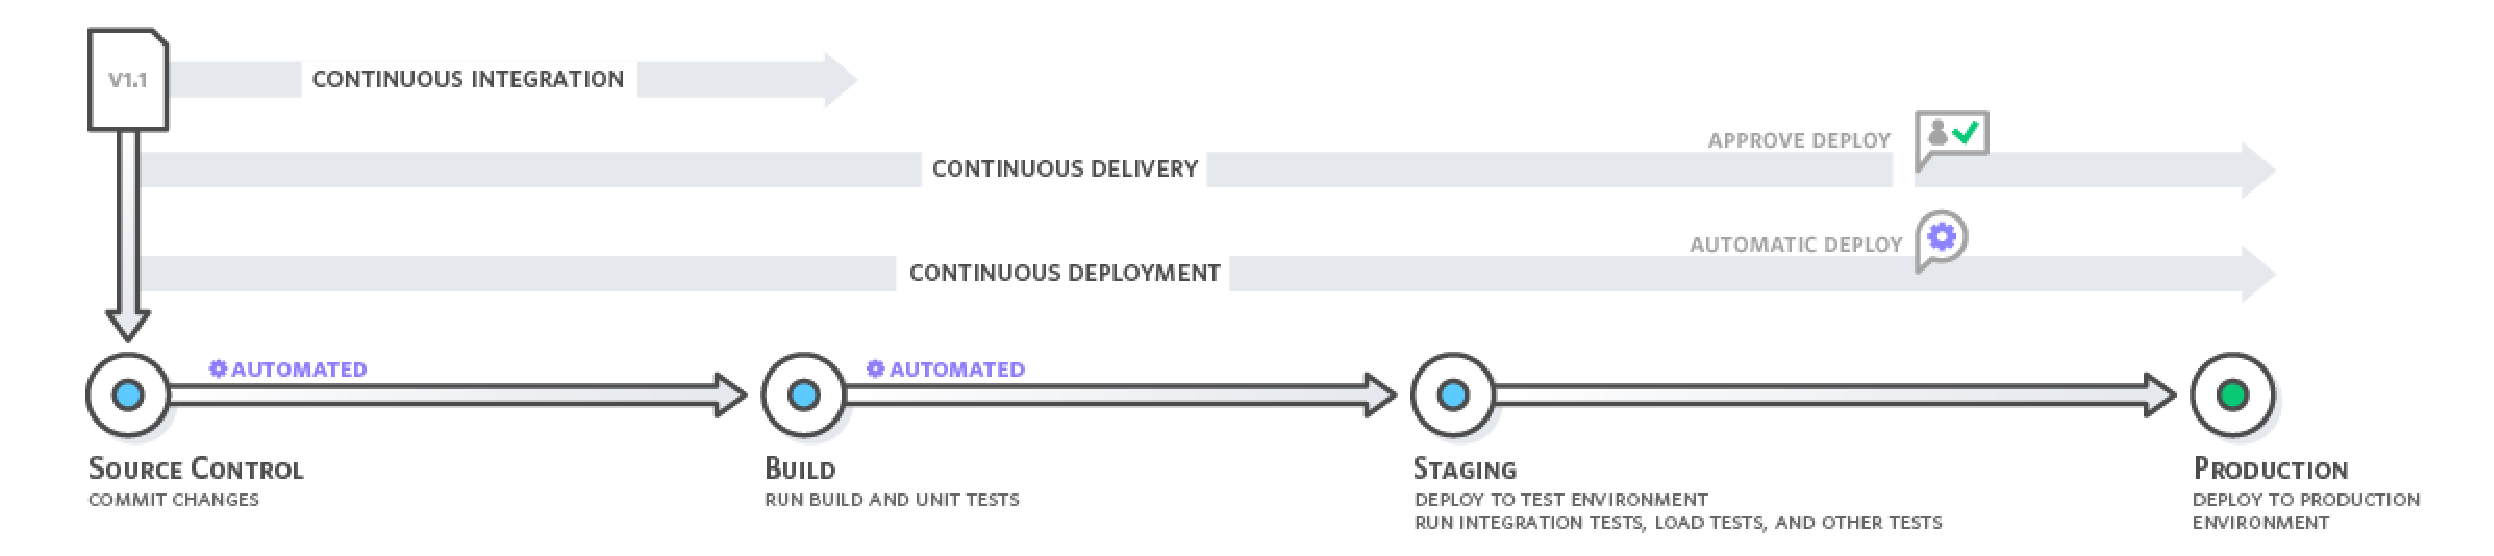
\includegraphics[width=\linewidth]{bibliografia/Imagenes/awsEC.eps}
    \caption{Diagrama de entregas continuas, tomado de \cite{awsEC}}
\end{figure}

Para lograr el objetivo de la integración continua y las entregas continuas existen diversas herramientas, dando mención a algunas estas son:

\begin{itemize}
    \item Terraform (Aprovisionamiento de infraestructura)
    \item CircleCI
    \item TravisCI
    \item Jenkins
    \item AWS Pipeline
\end{itemize}

\subsection{Versionamiento semántico}

Es un conjunto de reglas definidas para el control de versiones de un software y sus dependencias, que permite observar a grandes rasgos cambios y consecuencias al momento de definir o actualizar una dependencia, de acuerdo al autor Tom Preston-Werner en la web oficial \cite{semver} las reglas permiten definir:

Cómo asignar y cómo aumentar los números de versión. Para que este sistema funcione, tienes que declarar primero un API pública. Esto puede consistir en documentación o ser explicitado en el código mismo. De cualquier forma, es importante que esta API sea clara y precisa. Una vez que identificaste tu API pública, comunicas cambios a ella con aumentos específicos al número de versión. Considera un formato de versión del tipo X.Y.Z (Major.Minor.Patch) Los arreglos de bugs que no cambian el API incrementan el patch, los cambios y adiciones que no rompen la compatibilidad de las dependencias anteriores incrementan el minor, y los cambios que rompen la compatibilidad incrementan el major.

Este tipo de prácticas permiten evitar caer en dos problemas definidos por el autor, el primero el bloqueo de versiones (no se puede actualizar una pieza de software sin tener que actualizar todos los que dependen de la misma) o promiscuidad de versiones (asumir más compatibilidad con versiones futuras de lo razonable). Las reglas así mismo están documentadas en la web oficial.

\subsection{CircleCI}

CircleCI \cite {circleci} es una plataforma de CI/CD en la nube para la automatización de canales. Desde la interfaz de CircleCI se pueden pueden asociar repositorios de  GitHub. La el flujo de un canal es definida en un archivo de configuración YAML.

A continuación se definen algunos conceptos fundamentales para construir un canal en circleCI:

\begin{itemize}
	\item Step(Paso): Un comando que se ejecuta dentro de un trabajo.
	\item Job(Trabajo): Conjunto de pasos que se ejecutan en una sola unidad (un contenedor, una máquina).
	\item Workflow(Canal): Orden de los trabajos con sus respectivas reglas de ejecución.
\end{itemize}

\begin{figure}[H]
	\centering
	\includegraphics[width=\linewidth]{bibliografia/Imagenes/job.PNG}
	\caption{Un boceto de la configuración de un trabajo para pruebas unitarias}
	\label{jobcircle}
\end{figure}

Un trabajo requiere un conjunto de pasos y un contenedor (donde se ejecutan todos los pasos), como se ve en la figura \ref{jobcircle} ``Test'' es un trabajo que prepara la máquina y ejecuta las pruebas unitarias. La falla o interrupción de un trabajo detiene el flujo del canal (o flujo de trabajo) y es notificado en la interfaz de circleCI y Github para evitar su integración.

\begin {figure} [H]
\centering
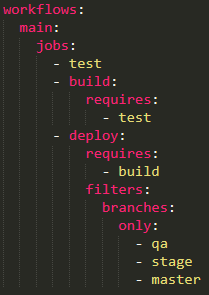
\includegraphics [width=0.5\linewidth]{bibliografia/Imagenes/workflow.PNG}
\caption{Ejemplo de un flujo de trabajo}
\label{workflow}
\end {figure}

En la figura \ref{workflow} se define un flujo de trabajo en el cual se definen una serie de filtros y atributos para determinar el orden y los pasos por cada rama

\subsubsection {Orb}

CircleCI \cite {circleci} define orb como ``fragmentos de código reutilizables que ayudan a automatizar los procesos repetidos''. Orbs permite reducir los pasos y la configuración simplemente llamando a un trabajo determinado (ya definido en el orb) en el flujo de trabajo agregando solo atributos adicionales, filtros o variables de entorno si es necesario. Como resultado, los orbes reducen la complejidad en una configuración y el tiempo para implementar nuevos flujos de trabajo en un canal.

\begin{figure}[H]
	\centering
	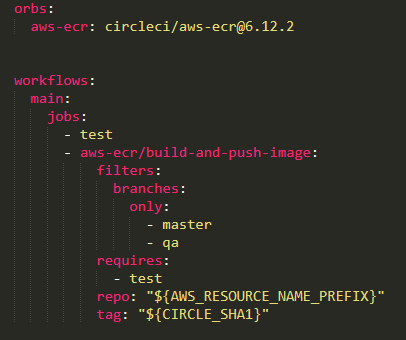
\includegraphics [width=0.4\linewidth]{bibliografia/Imagenes/orbexample.PNG}
	\caption {Ejemplo de la configuración de un orb}
	\label{orbexample}
\end{figure}

Los orb se definen en el atributo ``orbs'' en el archivo YAML del círculo CI. Un ejemplo es el orb ``aws-ecr/build-and-push-image'' que se usa en cuando se debe construir una imagen y subirla a AWS ECR (Elastic Container Registry), como se ve en la Figura \ref{orbexample}, no es necesario crear un trabajo ni escribir ningún comando, solo se necesitan los atributos necesarios para funcionar. Sin este orb, se deben agregar pasos adicionales como la instalación de AWS CLI y todo el proceso de creación de imágenes.

\subsection {IAC}

Matej Arta \ v {c} et al. definir una relación entre DevOps y la infraestructura como código (IaC):

\leftskip1.27cm\relax
\rightskip1.27cm\relax

DevOps promueve el uso de una noción típica de desarrollo de software, es decir, ``código fuente'', también para diseños de infraestructura, de modo que todo el conjunto de scripts, código de automatización y configuración, modelos, dependencias requeridas y parámetros de configuración operativa se pueden expresar utilizando el mismo idioma estándar. \cite{devopsiac}

\leftskip0cm\relax
\rightskip0cm\relax

IaC se encarga de todas las operaciones de la infraestructura (creación, actualización y eliminación) utilizando una definición de los recursos sin la intervención de desarrolladores o miembros de operaciones, por lo que ambos solo necesitan monitorear el estado de implementación o ser notificados si fue exitoso o no.
Terraform \cite{terraform} es una herramienta para IaC y utiliza una sintaxis para configuraciones que se llama HashiCorp Configuration Language (HCL), con esta sintaxis es posible describir la infraestructura en Amazon Web Services, Azure, Google Cloud, Kubernetes y otros proveedores.

\subsection {Terraform}
\subsubsection {Recursos y datos}
\subsubsection {Varibles}
\subsubsection {Modulos}
???
\subsection {SonarCloud}
???
\subsection {AWS}
???
\subsubsection {ECR}
???
\subsubsection {S3}
???
\subsubsection {ECS}
???
\subsubsection {Servicio}
???
\subsubsection {Definición de tarea}
???
\subsubsection {CloudWatch}
???
\subsubsection {Lambda}
???
\subsubsection {VPC}
???
\subsection {ElasticStack}
???
\subsubsection {Logstash}
???
\subsubsection {ElasticSearch}
???
\subsubsection {Kibana}
???
\subsection{SonarCloud}

SonarCloud es una plataforma para el análisis de código que detecta problemas de calidad del código fortaleciendo la capacidad de mantenimiento, confiabilidad y seguridad del código. De acuerdo con la página web oficial SonarCloud "utiliza técnicas de última generación en análisis de código estático para encontrar problemas, y posibles problemas, en el código" \cite{sonarcloud}.
Esta plataforma muestra el estado general del repositorio con frente a smells de código, puntos de acceso de seguridad, errores y vulnerabilidades.

\begin{figure}[H]
	\centering
	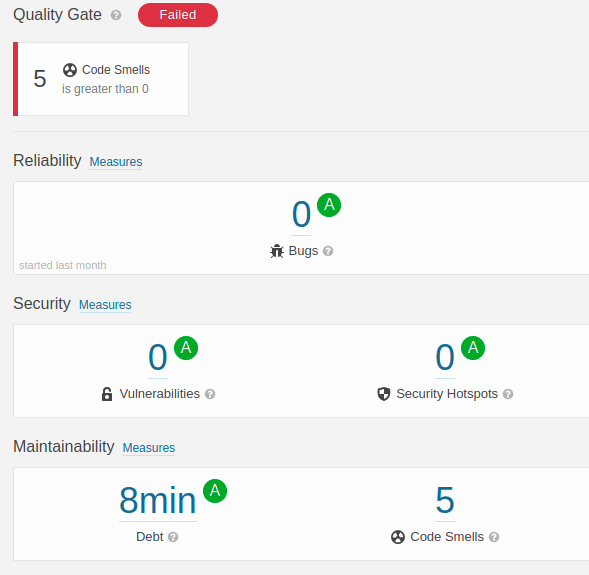
\includegraphics[width=0.8\textwidth]{bibliografia/Imagenes/SonarCloud.png}
	\caption{Interfaz de proyecto de sonarCloud}
	\label{sonarOne}
\end{figure}

En la figura \ref{sonarOne} observa la interfaz general de un proyecto donde se evidencia las vulnerabilidades encontradas. SonarCloud también permite localizar con exactitud el código que esta generando problemas junto con su motivo y posible solución como se contempla la figura \ref{sonarTwo}

\begin{figure}[H]
	\centering
	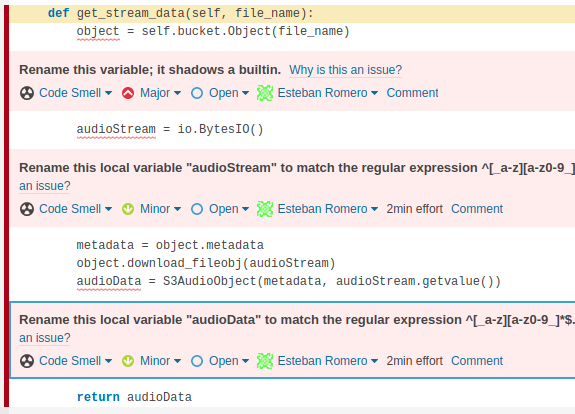
\includegraphics[width=0.8\textwidth]{bibliografia/Imagenes/Sonarbugs.png}
	\caption{Interfaz de código de SonarCloud}
	\label{sonarTwo}
\end{figure}

\chapter{Alcances y limitaciones}
\section{Alcances}
La planeación y despliegue de toda la infraestructura de servicios del sistema de detección de ruidos urbanos aplicando practicas de DevOps para la automatización de despliegues y pruebas unitarias, adicionalmente la integración de la infraestructura con estaciones receptoras de sonidos y herramientas de visualización de datos.
\section{Limitaciones}
\subsection{Tiempo}
\begin{itemize}
\item Tiempo de captura de audio
\item Tiempo de llegada de materiales para el proyecto
\end{itemize}
\subsection{Conectividad}
\begin{itemize}
\item Conectividad del centro de computación de alto desempeño ha sido interrumpida debido a fallas de servicio por largos periodos.
\item Disponibilidad en servicios de la nube los cuales tienen limitaciones de acuerdo al plan que se contrate
\item Fallas de servicio en hogares producidos por los respectivos proveedores de internet
\end{itemize}
\subsection{Espacio}
Ante la actual crisis sanitaria mundial existen limitaciones en materia de movilidad, acceso a los espacios (laboratorios del grupo de investigación) e interacción 

\chapter{Metodología}
\section{Enfoque}
El siguiente proyecto será abordado desde un enfoque empírico-analítico por los siguientes motivos:
\begin{itemize}
    \item Los algoritmos de inferencia basados en modelos de aprendizaje automático serán evaluados de acuerdo con métricas basadas en definiciones matemáticas que serán definidas en el proceso.
    \item La arquitectura tendrá un enfoque asociado al conocimiento empírico y analítico, ambas están incluidos en los siguientes aspectos: experiencia en el tema, los diseños con base a documentación y pruebas las cuales tendrán ciertos resultados cuantificables como lo son rendimiento en términos de latencia en red, tiempo de generación de resultados y otros que pueden variar de acuerdo a la arquitectura.
\end{itemize}
\section{Marco de trabajo}
Definir un marco de trabajo ágil que regirá en todo el proyecto que permita la entrega continua de componentes del sistema y su integración con el resto de acuerdo a unos requisitos que evolucionaran de forma continua. 
\section{Adquisición de archivos de audio}
Definir el software y hardware requerido para la recolección de archivos de audio desde diferentes puntos de la ciudad teniendo en cuenta la infraestructura (Equipos, Métodos de conectividad y transferencia de datos), estado del arte y conocimiento empírico. Adicionalmente verificar bases de datos y repositorios que contengan archivos de audio (en lo posible con etiquetas que definan las fuentes que aparecen en el mismo) para la realización de pruebas que serán necesarias posteriormente para la realización de pruebas de la arquitectura y el desarrollo.
\section{Selección de modelos de aprendizaje automático}
Definir las métricas para la selección de modelos de aprendizaje automático por medio de una exploración matemática con base en métodos de evaluación en algoritmos de aprendizaje automático. Posteriormente con base en las métricas definidas, seleccionar los modelos que serán implementados en el sistema y adaptarlos si es necesario, para lo cual se desarrollan interfaces y estándares que garanticen la adaptación del algoritmo al software.
\section{Arquitectura de software}
Definir una arquitectura híbrida con base en las arquitecturas REST, publicador/subscriptor y micro servicios que permita la inferencia, el almacenamiento de audio (si es requerido) y acceso a los resultados de forma concurrente con los mínimos retardos posibles por medio de una exploración en el tema y diseños de prueba, teniendo en cuenta prácticas que permitan un desarrollo resiliente, escalable y mantenible por medio de patrones de desarrollo, patrones de arquitectura, practicas de DevOps y versionamiento semántico. Adicionalmente se plantea la aplicación de servicios en la nube y modelos serverless que hacen parte del mismo dominio. A partir de ello definir tecnologías, metodología e iniciar el desarrollo.
\section{Desarrollo}
Desarrollar el software de acuerdo a la arquitectura, estándares y marco de trabajo definidos anteriormente, realizando en su momento prototipos que permitan verificar la capacidad del mismo de cumplir con la funciones requeridas, integrando mejora continua, prácticas de desarrollo de calidad y pruebas que garanticen escalabilidad, calidad de código, legibilidad del código y capacidad de refactorización.

\chapter{Desarrollo}
\section{Integración de prácticas de la cultura DevOPS al sistema de monitorio de ruido}
\subsection{Integración continua y despliegue continuo en el SMR}

Cada repositorio del Sistema NMS tiene dos ramas principales de git, Master y QA, la función de cada una es la siguiente:

\begin {itemize}
\item QA: esta es la rama principal para integrar todos los cambios en el código. Todo el código nuevo se prueba y analiza antes de poder enviarlo a esta rama.
\item Master: La rama de producción, donde el producto de software completa su último paso donde estará disponible para los consumidores.
\end {itemize}

\begin{figure}[H]
	\centering
	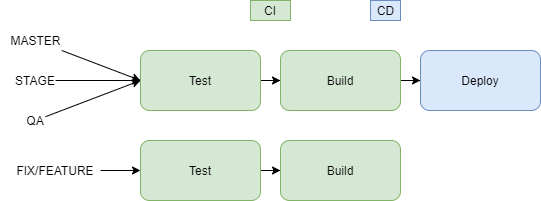
\includegraphics[width=\linewidth]{bibliografia/Imagenes/ci_cd branch Diagram.png}
	\caption{Diagrama de ramas y canales, el color indica que paso hace parte de la integración y el despliegue}
	\label{pipelines}
\end{figure}

Cada rama cuenta con  una serie de pasos como pueden observarse en la Figura \ref{pipelines} cuya función es la siguiente:
\begin{itemize}
\item Test: La aplicación de pruebas unitarias sobre todo el código para verificar la integridad del desarrollo y evitar que una funcionalidad pueda verse comprometida.
\item Build: El componente está preparado para ser implementado (crear una imagen, comprimir el código, construir el código, etc.).
\item Deploy: Despliega el componente en el entorno de desarrollo.
\end{itemize}

Como se ilustra en la Fig. \ref{pipelines}, las ramas principales (Master y QA) tienen un canal que incluye el despliegue, mientras que las ramas secundarias (con prefijo FIX/FEATURES) unicamente ejecutan los pasos de prueba y compilación, esto se debe en principio a que estas ramas son temporales y no tienen un ambiente de despliegue. Para cualquier integración es necesario que cualquier rama ejecute las pruebas unitarias y la compilación (en el caso de las ramas principales incluso el despliegue), de esta forma se verifica la integridad del código y se reduce el riesgo de llevar errores a ambientes superiores.


\subsection {Automatización de canales de los servicios del SMR}

\subsubsection {Servicios de inferencia}

En las Figuras \ref {pipelineA} y la Fig. \ref{pipelineB} se muestra el canal de los servicios de inferencia en circleCI, los trabajos se clasifican por etapa de la siguiente manera.

\begin {itemize}
	\item Test: Ejecuta pruebas unitarias y la verificación sonar de forma simultanea. Ambos pasos son requeridos para el build.
	\item Build: Compila y sube una imagen a AWS ECR.
	\item Deploy: Ejecuta un trabajo en un contenedor de terraform. Proporciona la infraestructura para los servicios de inferencia.
\end {itemize}

\begin{figure}[H]
\centering
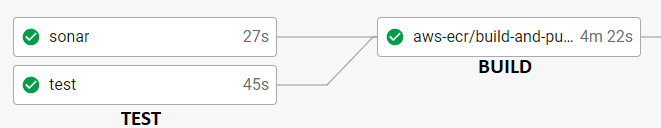
\includegraphics[width=0.8\linewidth]{bibliografia/Imagenes/inferencerpipelineA.PNG}
\caption {Parte A de la canalización del servicio de inferencia. Etapa de prueba y compilación}
\label {pipelineA}
\end {figure}

\begin{figure}[H]
\centering
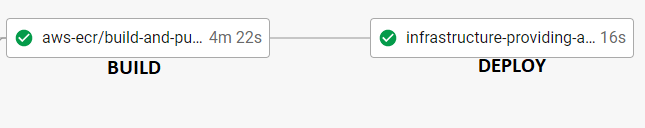
\includegraphics[width=0.8\linewidth]{bibliografia/Imagenes/inferencerpipelineB.PNG}
\caption {Canalización del servicio de inferencia, parte B, etapa de compilación e implementación}
\label {pipelineB}
\end {figure}


\subsubsection {Lambda para la publicación a Kafka}


En la Figura \ref{pipelineLambdaProducer} se muestra el canal para la Lambda de notificación a Kafka, los trabajos se clasifican por etapa de la siguiente manera.

\begin {itemize}
\item Build: Instala dependencias y genera un archivo ''zip´´ junto con el código que se almacena en el flujo de trabajo.
\item Deploy: Ejecuta un trabajo en un contenedor de terraform. Recupera ''zip´´ almacenado y lo despliega en AWS Lambda, adicionalmente crea el disparador desde S3.
\end {itemize}

\begin{figure}[H]
	\centering
	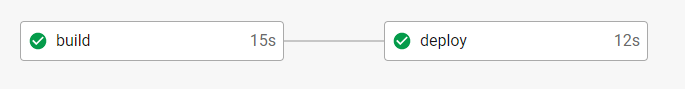
\includegraphics[width=1\linewidth]{bibliografia/Imagenes/lambdaProducerPipeline.PNG}
	\caption {Canalización del servicio lambda}
	\label {pipelineLambdaProducer}
\end {figure}


\subsubsection {Servicio de Logstash}

En la Figura \ref{pipelineKafkaLogstash} se ilustra el canal para el servicio de logstash, los trabajos se clasifican por etapa de la siguiente manera.

\begin {itemize}
\item Build: Se prepara la imagen para subirse a AWS ECR.
\item Deploy: Ejecuta un trabajo en un contenedor de terraform. Proporciona la infraestructura para el servicio de logstash.
\end {itemize}

\begin{figure}[H]
	\centering
	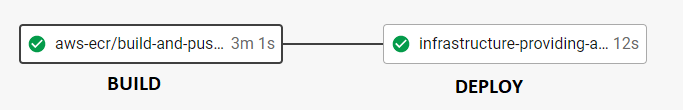
\includegraphics[width=1\linewidth]{bibliografia/Imagenes/kafkaLogstashPipeline.png}
	\caption {Canalización del servicio Logstash}
	\label {pipelineKafkaLogstash}
	\end {figure}

\subsection{Proveedor de terraform y backend}

Los proveedores son ``plugins que implementan tipos de recursos'' \cite{terraform}, permiten el uso de terraform con un proveedor en la nube. En el SMR se utiliza el plugin de AWS.

\begin{figure}[H]
	\centering
	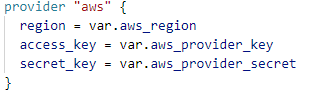
\includegraphics[width=0.7\textwidth]{bibliografia/Imagenes/providertf.PNG}
	\caption{AWS como proveedor en terraform}
	\label{providertf}
\end{figure}

Terraform mantiene un archivo de estado para mapear recursos a la configuración de terraform, seguimiento de metadatos y la mejora en el rendimiento en grandes infraestructuras \cite{terraform}. En el SMR cada servicio mantiene un archivo de estado almacenado en un bucket de S3, por lo que siempre esta disponible si se desea desplegar desde diferentes entornos de ejecución. la Figura \ref{backendtf}  muestra la configuración del backend para el servicio de inferencia (todos los servicios de SMR usan una configuración similar).

\begin{figure}[H]
	\centering
	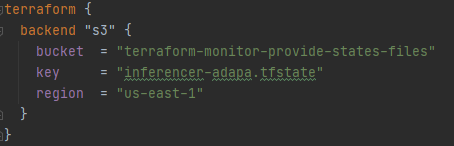
\includegraphics[width=0.8\textwidth]{bibliografia/Imagenes/backendtf.PNG}
	\caption{Definición del backend en terraform}
	\label{backendtf}
\end{figure}



\subsection{Despliegue de servicios de SMR con terraform}


La configuración detrás de cada componente del SMR involucra múltiples entidades o servicios de Amazon. La configuración de cada despliegue a mano reduce la eficiencia y puede llevar a errores o despliegues incompletos. En la Figura \ref{archcomponents} se mencionan los servicios utilizados y su relación.

\begin{figure}[H]
	\centering
	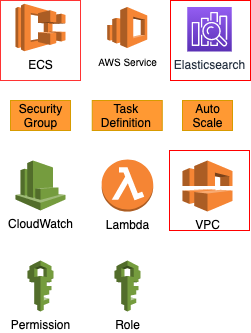
\includegraphics[width=0.80\textwidth]{bibliografia/Imagenes/Architecture Components.png}
	\caption{Componentes de AWS en el SMR}
	\label{archcomponents}
\end{figure}

Con terraform cada entidad en la figura \ref{archcomponents} es configurada una vez, luego su creación y despliegue es automático. Los componentes marcados con un recuadro rojo se llaman ``componentes compartidos'', lo que significa que son componentes a los que otras entidades están asociados, por este motivo tienen una configuración y un despliegue independiente.

\begin{figure}[H]
	\centering
	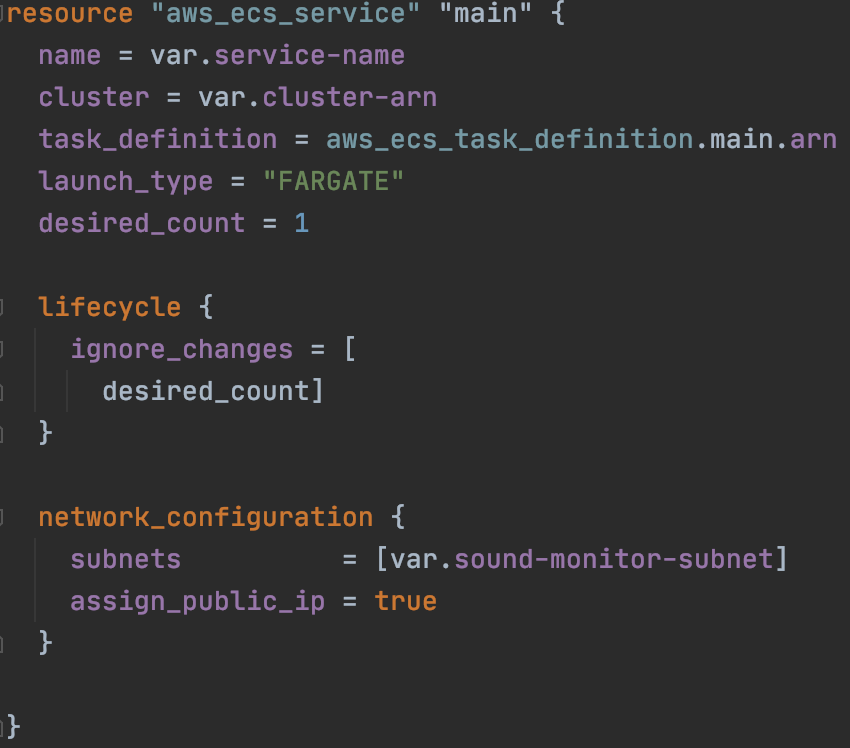
\includegraphics[width=0.8\textwidth]{bibliografia/Imagenes/infrastructure-providing.png}
	\caption{Configuración de un servicio de ECS para los servicios de inferencia}
	\label{ecsprovide}
\end{figure}

La figura \ref{ecsprovide} muestra la definición de un servicio utilizando terraform. Si algo es modificado en la configuración, terraform actualiza las entidades involucradas, sin crearlas nuevamente. En circleCI se puede monitorear el estado del despliegue de un servicio accediendo al trabajo de terraform como se muestra en la figura \ref{circleCITerraform}.

\begin{figure}[H]
	\centering
	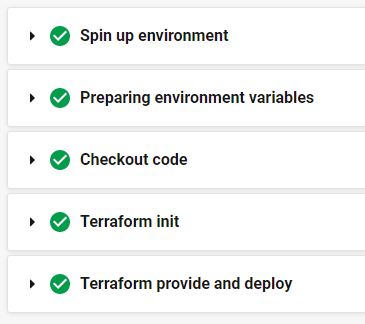
\includegraphics[width=0.7\textwidth]{bibliografia/Imagenes/circleCITerraformJob.png}
	\caption{Monitoreo de despliegue de terraform con circleCI}
	\label{circleCITerraform}
\end{figure}






\chapter{conclusiones}


\chapter{Recursos}

\section{Recursos materiales}
\begin{itemize}
    \item Servidor del CECAD de la Universidad Distrital con las siguientes características:
    \begin{itemize}
        \item Intel Core i7 9th
        \item 8 Gb RAM
        \item 250 GB Almacenamiento
    \end{itemize}
    \item Plataforma en la nube
        \begin{itemize}
        \item Amazon Web Services
        \item Google Cloud Computing Services
        \item Heroku
        \item Microsoft Azure
    \end{itemize}
    \item Sistemas de computo propios
    \item Raspberry Pi 3
\end{itemize}
\section{Recursos humanos}
\begin{itemize}
    \item Profesores directores de grupo y asociados
    \item Profesores de la facultad
    \item Miembros del grupo de investigación
\end{itemize}
\section{Presupuesto total del proyecto}

Para este proyecto los fondos propios son todos aquellos asumidos por los autores del proyecto. Bonos son todos aquellos fondos otorgados por plataformas de servicios en la nube. En la figura \ref{presupuesto} se definen el panorama presupuestal del proyecto.
\begin{figure}[H]
    \centering
    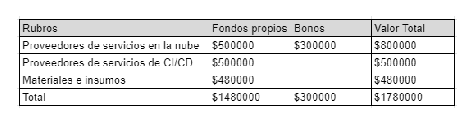
\includegraphics[width=\linewidth]{secciones/Imagenes/presupuesto.eps}
    \caption{}
    \label{presupuesto}
\end{figure}
En la figura \ref{Bonos} se precisa la procedencia de los bonos.
\begin{figure}[H]
    \centering
    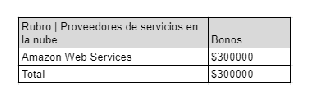
\includegraphics[width=\linewidth]{secciones/Imagenes/Bonos.eps}
    \caption{}
    \label{Bonos}
\end{figure}
En la figura \ref{materiales} se especifican los materiales e insumos requeridos para el desarrollo del proyecto.
\begin{figure}[H]
    \centering
    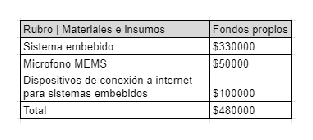
\includegraphics[width=\linewidth]{secciones/Imagenes/Materiales.eps}
    \caption{}
    \label{materiales}
\end{figure}
\newpage
\section{Cronograma}
\begin{figure}[H]
    \centering
    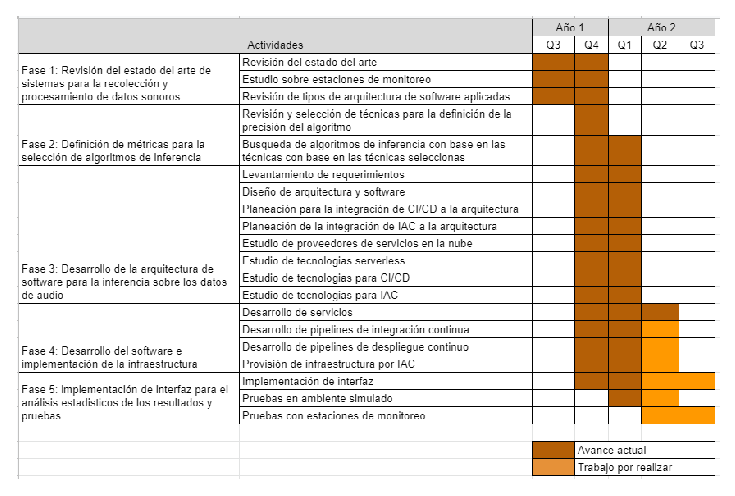
\includegraphics[width=\linewidth]{secciones/Imagenes/cronograma.eps}
    \caption{}
    \label{fig:my_label}
\end{figure}
\newpage

\medskip

\printbibliography

\end{document}

